\chapter{基本的事項}\label{ux57faux672cux7684ux4e8bux9805}

\section{my\_help}\label{my_help}

\subsection{my\_helpの目的}\label{my_helpux306eux76eeux7684}

my
helpとは,ユーザー独自のマニュアルを作成することができるユーザメモソフトである.これは,terminalだけを用いて簡単に起動,編集,削除などをすることができるため,非常に便利である.さらに,そのマニュアルは自分ですぐに編集,参照することができるので,メモとしての機能も果たし
ている.これにより,プログラミング初心者が,頻繁に使うコマンドやキーバインドなどをいちいちweb
browserを立ち上げて調べるのではなく,terminal上で即座に取得できるため,プログラム開発を集中することが期待される.

メモやtodoリストの作成が行えることや,保存場所を共通化することでどこでも立ち上げることができることなど,emacsのorg-modeと類似している点がいくつか存在する.しかし,明確な相違点も存在する.org-modeはemacsを起動させなければならないが,my
helpはemacsを起動させる必要がなくterminalで編集することが可能である.また,org-modeを使用するとなるとorg-mode独自のコマンドを学ぶ必要があり,学習コストがかかってしまう.my\_helpにはその必要がなく,非常に単純な操作でアプリを使用することができるので,org-modeの使い方を理解していない初心者にとって使いやすいものとなっている.

また,アプリやプログラミング言語などの正式なマニュアルは英語で書かれていることが多く,初心者には理解するのが困難である.my\_helpを使用すれば,自分なりのマニュアルを作成することができるので,仕様を噛み砕いて理解することが可能である.tarminal上でいつでもメモを参照できるため,どこにメモをしたかを忘れるリスクも軽減される.

\subsection{使用法}\label{ux4f7fux7528ux6cd5}

インストールする方法だが,gemの標準とは少し方法が異なっている.
まず,githubにあるmy
helpのリポジトリをフォーク,クローンすることでローカル(ネットワークに繋がれていない環境)でもmy
helpを操作することができるようになる.

\begin{quote}
git clone git@github.com:daddygongon/my\_help.git
\end{quote}
これ以降の作業はbundleにて行っていく.

\begin{quote}
bundle update
\end{quote}
を実行することでmy\_help.gemspecに記述されている必要なgemsがbundleされる.ここでCould
not locate
Gemfileとエラーが出た場合は、Gemfileのある場所を探し、その配下に移動してから再びコマンドを入力する.

\begin{quote}
bundle exec exe/my\_help
\end{quote}
でmy
helpに用意されているコマンドを参照することができる.デフォルトでemacs
helpというemacsのヘルプが用意されている.これはemacs
helpの他に,省略形のe\_hでも表示されるようになっている.

次に,独自のヘルプを作成する方法であるが,まず,

\begin{quote}
bundle exec exe/my\_help -i new\_help
\end{quote}
とすることでnew
helpという名前のヘルプが作成され,そこにテンプレートが格納される.また,

\begin{quote}
bundle exec exe/my\_help -e new\_help
\end{quote}
で,自分の好きなように編集することができる.ヘルプが完成したら,

\begin{quote}
bundle exec exe/my\_help -m
\end{quote}
とすることでexeディレクトリにnew helpが追加され,new
help,n\_hが使用可能になるという手順である.

\section{optparse}\label{optparse}

今回の研究対象のmy
helpは,optparseで実装されている.optparseはRubyの標準ライブラリであり,Rubyでコマンドラインのオプションを操作するためのライブラリである{[}1{]}.optparseが操作するオプションは,下記のonメソッドで設定する.

\begin{screen}
{\small
\begin{verbatim}
def execute
  @argv << ’--help’ if @argv.size==0
  command_parser = OptionParser.new do |opt|
    opt.on(’-v’, ’--version’,’show\UTF{2423}program\UTF{2423}Version.’ ) { |v|
      opt.version = MyHelp::VERSION
      puts opt.ver
    }
    opt.on(’-l’, ’--list’, ’list\UTF{2423}specific\UTF{2423}helps’){list_helps}
    #中略
  end
  #中略
end
    
def list_helps
#中略
end
#後略
\end{verbatim}}
\end{screen}


第1引数はショートオプションで,-aや-dのような形で設定する.同様にして,第2引数はロングオプションを表し,-\/-addや-\/-deleteのように,第3引数はそのオプションの説明文で,helpで表示される説明文を設定する.後ろのブロックには,そのオプションが指定された場合に実行されるコードを記述する
{[}2{]}.しかしこのライブラリでは自然言語に近い,ハイフンなしのサブコマンドを実装するには相当な書き換えが必要となる.

メソッドの引数でオプションを定義し,引数が指定された時の処理をブロックで記述する.ブロックの引数にはオプションが指定されたことを示すtrueが渡される.onメソッドが呼ばれた時点ではオプションは実行されず,定義されるだけである.parseが呼ばれた際,コマンドラインにオプションが登録されていれば実行される.

オプション定義の際,スペースの後に任意の文字を追加すると,そのオプションは引数を受け取るオプションになる.その文字に{[}{]}をつけることで引数は必須でなくなる.また引数がハイフンで始まる場合,オプションとの間にハイフンを2つ挟むことで引数として認識される.

helpとversionのサブコマンドはデフォルトで作成される.

\section{thor}\label{thor}

本研究ではoptparseの代わりのライブラリとしてThorの採用を検討する.Thorは,コマンドラインツールの作成を支援するライブラリであり,gitやbundlerのようにサブコマンドを含むコマンドラインツールを簡単に作成することができる
{[}3{]}.Thorには以下のような特徴がある. 1.
コマンドラインオプションのパーズやサブコマンドごとのヘルプを作るなどの面倒な作業を簡単にこなすことができ,手早くビルドツールや実行可能なコマンドを作成できる
{[}4{]}. 1. 特殊なDSL(Domain Specific
Language)を使わずにメソッドを定義することで処理を記述するため,テストを行いやすい
{[}4{]}. 1.
optparseでは作成することが困難な,マイナスを伴わない(自然言語に近い)サブコマンドを実装することが可能である.

\begin{screen}
{\small
\begin{verbatim}
desc 'list, --list', 'list specific helps'
    map "--list" => "list"
    def list
      print "Specific help file:\n"
      local_help_entries.each{|file|
        file_path=File.join(@local_help_dir,file)
        help = YAML.load(File.read(file_path))
        print "  #{file}\t:#{help[:head][0]}\n"
      }
    end
end
\end{verbatim}}
\end{screen}


optparseではonメソッドでコマンドの登録を行い,その後のdefでコマンドの振る舞いを定義している.それに対してThorは登録と定義を同時に行うことが可能である.また,Thorを継承したクラスのパブリックメソッドがそのままコマンドになるので非常に簡単にコマンドを作成することが可能である.Thorはコマンドを作成した時点で自動的にヘルプを生成し,コマンドを指定せずにコマンドラインアプリを実行するとヘルプを表示する.

\begin{figure}[H]
\centering
\begin{center}
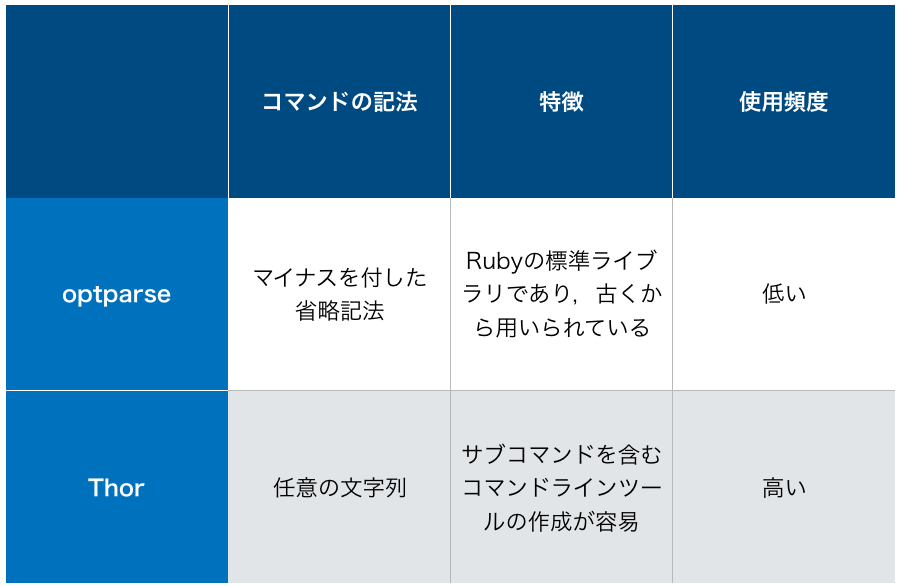
\includegraphics[width=150mm]{../.././figs/opt_thor.png}
\end{center}
\caption{optparse とThor の比較. \label{opt_thor}}

\label{fig:This}
\end{figure}

    \section{option}\label{option}

今日,複雑な機能を持つコマンドが増加している.そのようなコマンドは,オプション(サブコマンド)を使用することで適切な動作を実行することが可能になる.例えばgitコマンドはオプションなしでは意味をなさない.オプションでどのような動作をするかが決まるので,オプションを入力することで正常に動作するのである.

そもそも,オプションにはショートオプションとロングオプションの2種類がある.ショートオプションはハイフンの後に英字1字を付けた形式のもので,-aや-vなどといったものがショートオプションである.また,ショートオプションは2つ以上のオプションを1つにまとめて実行することもできる.例えば,-l,-a,-tの3つのオプションを1つにまとめて-latとして実行することが可能である.それに対してロングオプションは,ハイフン2つの後に英字2字以上を付けることができる形式である.例えば-\/-allや-\/-versionなどである.ロングオプションは英字を2字以上使用することができるので,どのようなオプションであるかを明確にするために一般的にフルワードが採用されている.-\/-no-の形にすることで否定形のオプションを作成することも可能である.ロングオプションはショートオプションのように複数のオプションを1つにまとめることは不可能であり,1つ1つをスペースで区切る必要がある.

ショートオプションを設定する際,英字1文字しか使用することができないので基本的には対応づけられたロングオプション(そのオプションがどのような動作を行うのかを表す単語)の頭文字であることが多く,慣れている人であればショートオプションを使うことで素早くアプリケーションを動かすことが可能である.しかし,用いるアプリが1つであるとは限らないし,全てのアプリのショートオプションを統一するのも困難である.またinitialとinstallなど,頭文字が重複してしまう2つのオプションがある場合,-iというショートオプションがinitialを意味するのかinstallを意味するのかを判断するのは,初心者には容易ではなく,混乱を引き起こしかねない.そのため,ヒューマンエラーを引き起こしてしまったり,学習コストがかかってしまったりすることがある.

ショートオプションの場合,複数のオプションを一つにまとめることができると記述したが,これは引数を必要としないオプションの場合である.引数を必要とするオプションの場合,2文字目以降の英字は引数扱いになってしまう.例えば上に示した-latにおいて,-lが引数を必要とするオプションであれば,-latはatという引数が与えられた-lという風に解釈されてしまうので注意が必要である.そういった点においてもショートオプションは初心者にとって扱いにくい形式であると言える.

Command line
applicationのオプションの記述方法には幾つもの流儀があるようで
何らかの標準があるわけではない.
しかし,それら全てに対応することはできず,なんらかの
基準に従ってオプション記法を解釈する必要がある.

ここでは, "Build awesome command-line application in ruby 2"に従って
オプション記法と用語をまとめておく.

コマンドラインの基本形は,

\begin{quote}
ls -lat dir\_name
\end{quote}
というように

\begin{quote}
executabel options arguments
\end{quote}
での形であった.これは,GNU標準に基本構造が記載されている.

その後,幾つかのswitchやflagを組み合わせて,複雑な
命令を解釈できるようにするに従って,

\begin{quote}
grep -\/-igonre-case -C 4 "some string" /tmp
\end{quote}
などとほぼ呪文のような形態となってきた.

その後,command line suiteと呼ばれる一群のcommand line
applicationが登場した.典型的なのはgitである{[}5{]}.

gitはlinuxのバックアップを分散処理するために, Linus
Torvaldsが開発したものであるが,いくつもの
機能に従ってそれぞれ個別のコマンドが用意されていた.
それぞれ,git-commitとかgit-fetchなどであった.
それがある時,すべてをまとめてsuiteとして
パッケージし直され,1つのまとまったcommandとして提供された.
すなわち,git commitやgit fetchなどである{[}6{]}.

    